\documentclass[a4paper, 11pt,oneside]{article}
\usepackage[
  top=1.5cm,
  bottom=1cm,
  left=2cm,
  right=1.5cm,
  headheight=25.22153pt, % as per the warning by fancyhdr
  includehead,includefoot,
  heightrounded, % to avoid spurious underfull messages
]{geometry} 

\usepackage{pdflscape}
\usepackage[T1]{fontenc}
\usepackage{microtype}
\usepackage{fancyhdr}
\usepackage{fancyvrb}
\usepackage{lipsum}
\usepackage{url}
\usepackage{listings}
\usepackage{lastpage}
\usepackage{enumitem}
\usepackage{datetime}
\usepackage{amsthm}
\usepackage{graphicx}
\usepackage{hyperref}
\usepackage{caption}
\usepackage[newfloat]{minted}
\usepackage{float}

\captionsetup[listing]{position=bottom}

\settimeformat{hhmmsstime}
\yyyymmdddate

\pagestyle{fancy}
\fancyhf{} % clear all fields

\pagestyle{fancy}
\lhead{CMSC 132: Computer Architecture \\ First Semester 2020-2021}
\rhead{Institute of Computer Science \\ University of the 
Philippines Los Banos}
\rfoot{$\copyright$JACHermocilla (CC NC-BY-SA 4.0)}
%\cfoot{Enjoy!:)}
\cfoot{\thepage\ of \pageref{LastPage}}
\lfoot{Revision: \today\ \currenttime}
%\rfoot{https://jachermocilla.org/teaching/125}
\renewcommand{\headrulewidth}{0.4pt}
\renewcommand{\footrulewidth}{0.4pt}

\begin{document}

\begin{center}
	{\LARGE \textbf{Instruction Set Architecture Design and Implementation}}
\end{center}

\section*{Learning Outcomes}
   At the end of this lab, you should be able to:
   \begin{enumerate}[itemsep=0pt,parsep=0pt]
   	   \item understand and modify a simple ISA and its implementation;
       \item write a simple assembler
   \end{enumerate}   
\tableofcontents

\section{Resources}
\begin{itemize}
	\item Video: \href{https://youtu.be/CzyXb_T-xgU}{https://youtu.be/CzyXb\_T-xgU}.
	\item Source Codes: \href{https://git.io/JU3al}{https://git.io/JU3al}
	\item Online VHDL Tool: \href{https://www.edaplayground.com/home}
	{https://www.edaplayground.com/home}
\end{itemize}	

\section{Discussion}
The \textbf{processor(CPU)} is composed of the \textbf{datapath} and 
\textbf{control}. In the previous labs, you learned that combinational and 
sequential circuit elements are used as building blocks to create the 
functional components of the datapath and control. Examples of these functional 
elements include the \textbf{ALU, Register File, Program Counter, and Memory}. 
You also learned that a \textbf{clock} drives the execution forward and control 
is implemented using a \textbf{finite state machines} for the 
\textbf{fetch-decode-execute} cycle. One question that we can answer next is: 
\textit{How do we program the CPU?}


\subsection{Instruction Set Architecture}
Instruction Set Architecture (ISA) is an \textbf{abstraction} between the 
hardware and the lowest-level software. It includes anything programmers need 
to know to make a binary machine language program work correctly. Typically it  
documents the set of instructions that can be performed by the 
processor, the number and name of available registers, the memory 
addressing modes, I/O, interrupt processing, etc \cite{CODARM}.

ISA allows computer designers to talk about functions indepedently from the 
hardware that performs them. This abstact interface enables many 
implementations (aka \textbf{microarchitectures}) of varying costs and 
performance to run identical software.

Examples of ISA include the \textbf{IA-32} and \textbf{x86-64}\cite{AMD64ISA} 
which are commonly used in desktop and laptops. For example, Intel implements 
these ISA in their Intel Core i5-8250U\cite{Corei5} product as \textbf{8th 
Generation aka Kaby Lake Refresh}\cite{KarbyLaKeR}. AMD also implements these 
ISA in the Ryzen 5000 \cite{Ryzen5000} as \textbf{4th Gen aka Zen 
3}\cite{Zen3}. There are other implementations(aka generations) that vary in 
their performance characteristics.

For mobile devices, a popular ISA is the \textbf{ARMv8 A64}\cite{ARMv8ISA}. 
MediaTek uses ARM's \textbf{Cortex-A73} and \textbf{Cortex-A53}\cite{CortexA73} 
implementations in their Octa-core Helio P70\cite{HelioP70}. Qualcomm also uses 
the same implementations in their Kryo 240 processor for Snapdragon 460 Mobile 
Platform\cite{Snapdragon460}.

\subsection{Application Binary Interface}
Application Binary Interface (ABI) is a combination of the basic instruction 
set and the operating system interface provided for application 
programmers\cite{CODARM}. 

For general-purpose use such a desktops and laptops, programming a processor 
using only the basic instruction set is insufficient. Thus, operating systems 
perform an important role in the management and efficient use of hardware 
resources in addition to making it easier for users to use a computer. 

ABI describes function-calling conventions, parameter passing, sizes of 
C data types, executable file formats (ELF, PE). Examples are the IA-32 and 
\textbf{x86-64 System V ABI}\cite{x64ABI} which are used in Linux and other 
Unix-type 
operating systems. Windows has its own ABI called \textbf{x64 
ABI}\cite{Winx64ABI}. Android supports different ABIs\cite{AndroidABI}.


\subsection{ISA Taxonomy}
We can categorize ISAs based on where operands in instructions are stored.
\textbf{Stack-based} ISAs uses a stack(LIFO) where operations are performed on 
the operands on the top of the stack. In \textbf{accumulator-based} ISAs, one 
register is designated as the \textit{accumulator} and its use in operations is 
implied. Modern ISAs are \textbf{general purpose} where operands are explicitly 
named in the instruction. In this category, operations can be 
register-to-register, register-to-memory, or memory-to-register.

\subsection{Considerations in ISA Design}
\begin{itemize}
\item \textit{Types/Class of instructions(Operations in the instruction set)} - 
arithmetic/logic, data movement, branching/control flow, I/O, etc.
\item \textit{Types and sizes of operands (in bits)} - 8, 16, 32, 64, 128, 
floating point 
\item \textit{Addressing modes} - register, direct, indirect, immediate, etc.
\item \textit{Addressing memory} - byte-addressable, word-addressable, 
endian-ness
\item \textit{Encoding and Instruction Formats} - opcode field, addresses 
field, mode 
field
\item \textit{Compiler-related issues} - optimization features
\end{itemize}

\subsection{Example Instruction Formats}
Figure \ref{fig:x86-64} and Figure \ref{fig:armv8}  are the instruction formats 
for x86-64 and ARMv8, taken from their documentation manuals. The x86-64 format 
is more complex than that of the ARMv8 with variable widths in terms of number 
of bits for the opcode.

\begin{figure}[H]
	\begin{center}
	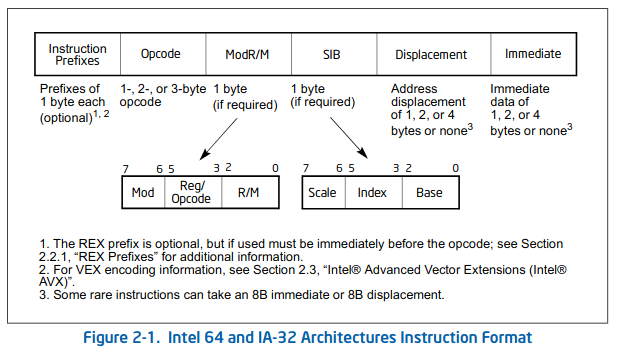
\includegraphics[width=4in]{x86-64.png}
	\caption{x86-64 Instruction Format (CISC).}
	\label{fig:x86-64} 
	\end{center}
\end{figure}

\begin{figure}[H]
	\begin{center}
	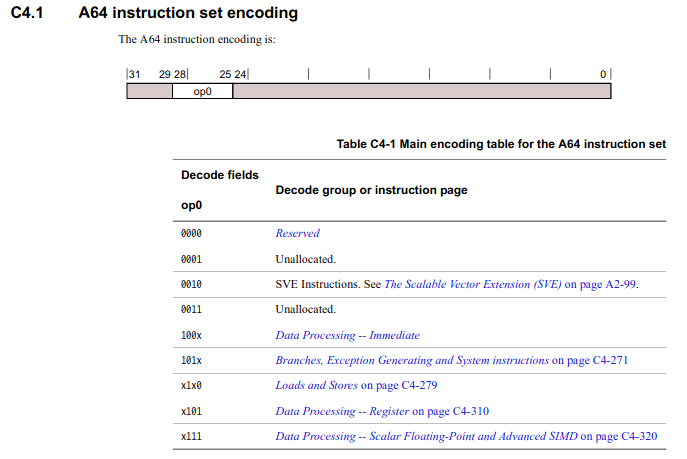
\includegraphics[width=4in]{armv8.png}
	\caption{ARMv8 Instruction Format (RISC).}
	\label{fig:armv8} 
	\end{center}
\end{figure}

\subsection{TOMA: The Optimal Machine Architecture}
Let us look at the design of a simple ISA which we will call TOMA.

\subsubsection{Features}
\begin{itemize}
\item Four 8-bit registers named \mintinline{asm}{$s0, $s1, $s2, $s3} when 
used in assembly code
\item Instruction memory (IM) is 8 bytes(8x8), address line is 3 bits
\item Three-bit Program Counter (PC)
\item Single-cycle - completes instruction execution in one clock cycle
\item Supports the following instructions: \mintinline{asm}{and, add, sub, 
addi}
\item No data memory, thus has no load and store instructions
\item No control transfer instructions
\end{itemize}

\subsubsection{Instruction Format}
The size of an instruction in TOMA is 8 bits divided into the configuration 
shown in Figure \ref{fig:ins_format}.

\begin{figure}[H]
	\begin{center}
	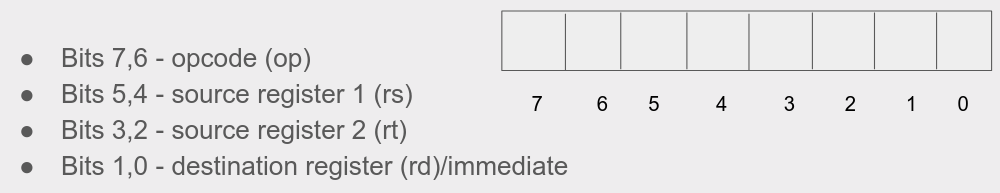
\includegraphics[width=4.5in]{ins_format.png}
	\caption{TOMA instruction format.}
	\label{fig:ins_format} 
	\end{center}
\end{figure}

\subsubsection{Supported Instructions}
\begin{listing}[H]
\caption{Supported Instructions in TOMA.}
\label{code:instructions}
\begin{minted}[frame=single,framesep=10pt]{vhdl}
and : rd <= rs AND rt           (op=00)
add : rd <= rs + rt             (op=01)
sub : rd <= rs -  rt            (op=10)
addi : rs <= rt + immediate     (op=11)
\end{minted}
\end{listing}


\subsubsection{Assembly Language}


The syntax for the assembly language is shown in Listing \ref{code:assembly}.

\begin{listing}[H]
\caption{Assembly language syntax.}
\label{code:assembly}
\begin{minted}[frame=single,framesep=10pt]{nasm}
<instruction> <dst>, <src1>, <src2/imm>
\end{minted}
\end{listing}


\begin{listing}[H]
\caption{Example assembly code and corresponding machine code.}
\label{code:assembly_sample}
\begin{minted}[frame=single,framesep=10pt]{nasm}
addi $s0, $s0, 2         ; 11000010b, 0xC2
addi $s1, $s1, 1         ; 11010101b, 0xD5
addi $s2, $s2, 3         ; 11101011b, 0xEB
add $s3, $s0, $s1        ; 01000111b, 0x47
sub $s0, $s2, $s3        ; 10101100b, 0xAC
\end{minted}
\end{listing}

\subsection{REDHORSE 500: An implementation of TOMA}

\subsubsection{Features}
\begin{itemize}
\item Implements the TOMA ISA in VHDL
\item Clocked at 100MHz
\end{itemize}

\subsubsection{Processor}
The interface to the processor is shown in Listing \ref{code:processor} which 
shows that it has one input which is the clock and two outputs. Figure 
\ref{fig:redhorse500} shows the complete wiring of the functional components. 
We will discuss the operation of the individual components in the remaining 
subsections. 

\begin{listing}[H]
\caption{Interface to the processor.}
\label{code:processor}
\begin{minted}[frame=single,framesep=10pt]{vhdl}
ENTITY Processor IS 
    PORT
    (
        clk :  IN  STD_LOGIC;
        current_instruction :  OUT  STD_LOGIC_VECTOR(2 DOWNTO 0);
        value :  OUT  STD_LOGIC_VECTOR(7 DOWNTO 0)
    );
END Processor;
\end{minted}
\end{listing}

\begin{landscape}
\thispagestyle{plain}
\begin{figure}[H]
	\begin{center}
	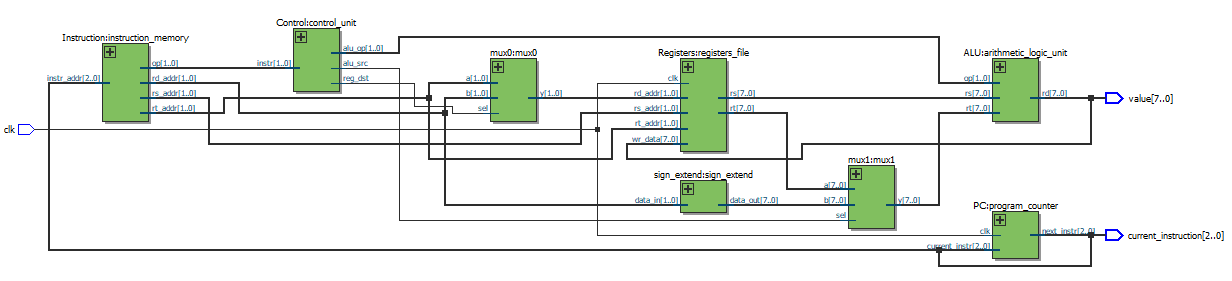
\includegraphics[width=10.5in]{redhorse500.png}
	\caption{Wiring of the different functional components of REDHORSE 500.}
	\label{fig:redhorse500} 
	\end{center}
\end{figure}
\end{landscape}
%%[width=10in]

\subsubsection{Program Counter}
The Program Counter will generate the address of the next instruction. It adds 
1 to the value of \mintinline{vhdl}{current_instr}.
\begin{listing}[H]
\caption{Interface to the Program Counter.}
\label{code:pc}
\begin{minted}[frame=single,framesep=10pt]{vhdl}
entity PC is
  port(
    clk           : in std_logic;
    current_instr : in std_logic_vector(2 downto 0);   -- current instruction
    next_instr    : out std_logic_vector(2 downto 0)   -- next instruction
  );
end PC;
\end{minted}
\end{listing}

\begin{figure}[H]
	\begin{center}
	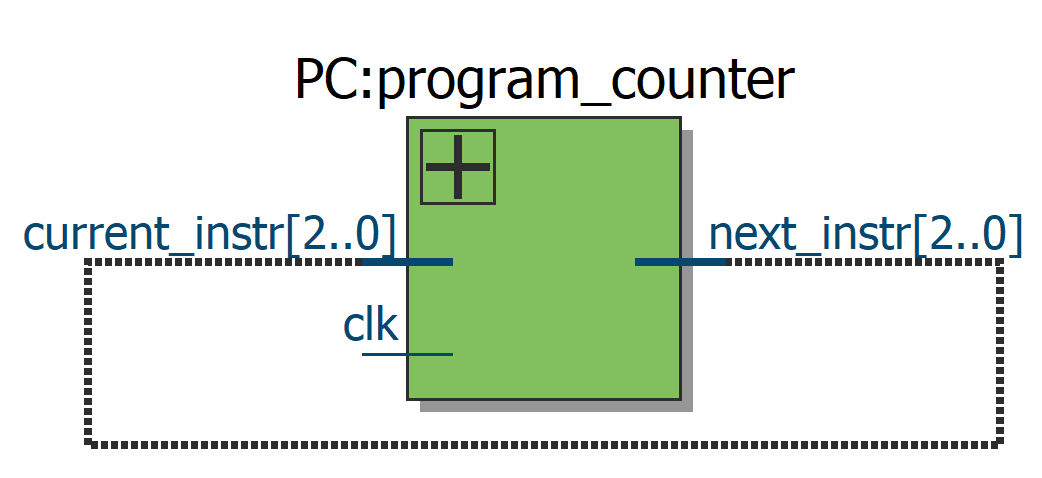
\includegraphics[width=2in]{pc.png}
	\caption{Program Counter.}
	\label{fig:pc} 
	\end{center}
\end{figure}

\subsubsection{Instruction Memory}
Instruction Memory contains the instructions to be executed in an array of 
1-byte cells. It will decode the instruction specified by 
\mintinline{vhdl}{instr_addr}. The decode process will extract and output the 
different parts of the instruction: \mintinline{vhdl}{op}, 
\mintinline{vhdl}{rs_address}, \mintinline{vhdl}{rt_address}, 
\mintinline{vhdl}{rd_address/imm}.

\begin{listing}[H]
\caption{Interface to the Instruction Memory.}
\label{code:im}
\begin{minted}[frame=single,framesep=10pt]{vhdl}
entity Instruction is
  port(
    instr_addr : in std_logic_vector(2 downto 0);  -- instruction address

    op         : out std_logic_vector(1 downto 0); -- operation code
    rs_addr    : out std_logic_vector(1 downto 0); -- source register 1 addr    
    rt_addr    : out std_logic_vector(1 downto 0); -- source register 2 addr
    rd_addr    : out std_logic_vector(1 downto 0)  -- dest register addr
  );
end Instruction;


\end{minted}
\end{listing}

\begin{figure}[H]
	\begin{center}
	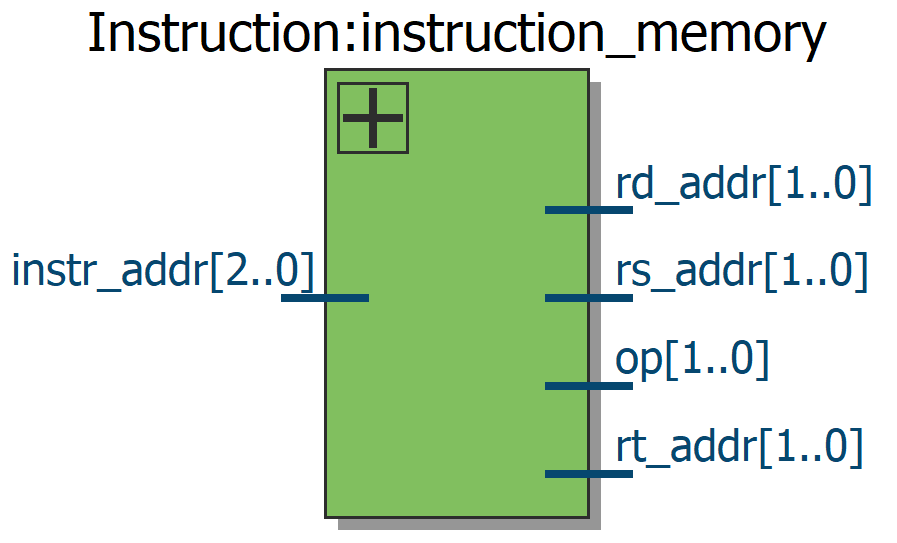
\includegraphics[width=2in]{im.png}
	\caption{Instruction Memory.}
	\label{fig:im} 
	\end{center}
\end{figure}

\begin{listing}[H]
\caption{Sample hard-coded instructions in the instruction memory.}
\label{code:im_code}
\begin{minted}[frame=single,framesep=10pt,linenos]{vhdl}
     constant instr : instruction_set := (
       "11000010",  -- addi $s0, $s0, 2
       "11010101",  -- addi $s1, $s1, 1
       "11101011",  -- addi $s2, $s2, 3
       "01000111",  -- add  $s3, $s0, $s1
       "10101100",  -- sub  $s0, $s2, $s3
       "00000000",
       "00000000",
       "00000000"
     );    
\end{minted}
\end{listing}


\subsubsection{Register File}
The Register File is composed of four 8-bit registers. The contents of the 
registers specified by \mintinline{vhdl}{rs_addr} and 
\mintinline{vhdl}{rt_addr} are the outputs \mintinline{vhdl}{rs} and 
\mintinline{vhdl}{rt}. At the falling edge of the clock, the data in 
\mintinline{vhdl}{wr_data} is written into the register 
specified by \mintinline{vhdl}{rd_addr}. The \mintinline{vhdl}{rd_addr} input 
will come from Mux0 in case the instruction is \mintinline{vhdl}{addi}(See 
Figure \ref{fig:redhorse500}).


\begin{listing}[H]
\caption{Interface to the Register File.}
\label{code:rf}
\begin{minted}[frame=single,framesep=10pt]{vhdl}
entity Registers is
  port(
    clk     : in std_logic;

    rs_addr : in std_logic_vector(1 downto 0);    -- source register 1 address
    rt_addr : in std_logic_vector(1 downto 0);    -- source register 2 address
    rd_addr : in std_logic_vector(1 downto 0);    -- destion register address
    wr_data : in std_logic_vector(7 downto 0);    -- write data to dest register

    rs      : out std_logic_vector(7 downto 0);   -- source register 1 value
    rt      : out std_logic_vector(7 downto 0)    -- source register 2 value
  );
end Registers;

\end{minted}
\end{listing}

\begin{figure}[H]
	\begin{center}
	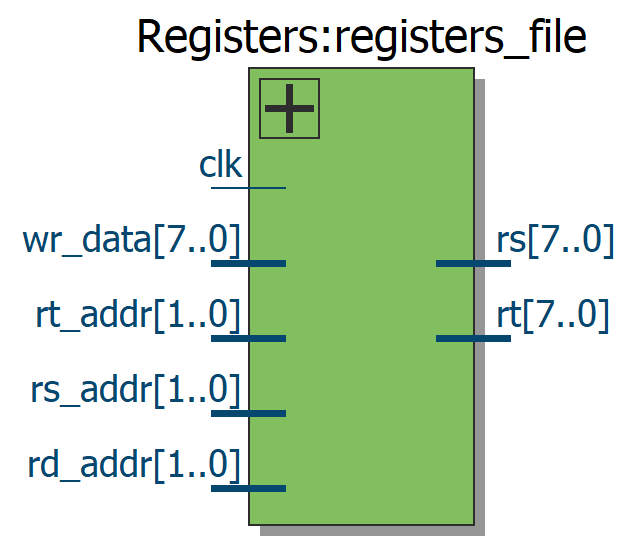
\includegraphics[width=2in]{rf.png}
	\caption{Register File.}
	\label{fig:rf} 
	\end{center}
\end{figure}

\begin{listing}[H]
\caption{Sample hard-coded initial values for the registers.}
\label{code:rf_values}
\begin{minted}[frame=single,framesep=10pt]{vhdl}
   signal reg: registerFile := (
    "00000001",
    "00000010",
    "00000011",
    "00000100"
);
\end{minted}
\end{listing}

\subsubsection{ALU}
The ALU performs the supported instructions depending on the opcode in 
\mintinline{vhdl}{op}. This is an 8-bit ALU so operations are performed on 
8-bit values. The inputs are in \mintinline{vhdl}{rs} and \mintinline{vhdl}{rt} 
and the results in \mintinline{vhdl}{rd}. \mintinline{vhdl}{rt} input will come 
form Mux1 in case the instruction is \mintinline{vhdl}{addi}(See Figure 
\ref{fig:redhorse500}).

\begin{listing}[H]
\caption{Interface to the ALU.}
\label{code:alu}
\begin{minted}[frame=single,framesep=10pt]{vhdl}
entity ALU is
  port(
    op  : in std_logic_vector(1 downto 0);   -- operation code

    rs  : in std_logic_vector(7 downto 0);   -- source register 1
    rt  : in std_logic_vector(7 downto 0);   -- source register 2
    rd  : out std_logic_vector(7 downto 0)   -- destination register
  );
end ALU;

\end{minted}
\end{listing}

\begin{figure}[H]
	\begin{center}
	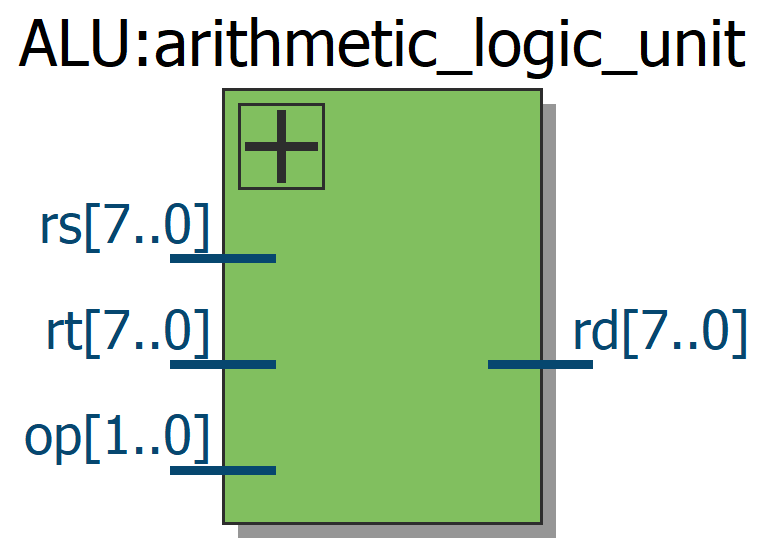
\includegraphics[width=2in]{alu.png}
	\caption{ALU.}
	\label{fig:alu} 
	\end{center}
\end{figure}

\subsubsection{Control Unit}
The Control Unit activates control lines depending on the opcode in 
\mintinline{vhdl}{instr}. It tells the ALU what operation to perform through 
the \mintinline{vhdl}{alu_op} line. A special case is 
the \mintinline{vhdl}{addi} instruction which activates the 
\mintinline{vhdl}{alu_src} and \mintinline{vhdl}{reg_dst} to adjust the 
inputs to the ALU and the Register File respectively (See Figure 
\ref{fig:redhorse500}). 


\begin{listing}[H]
\caption{Interface to the Control Unit.}
\label{code:control}
\begin{minted}[frame=single,framesep=10pt]{vhdl}
entity Control is
  port(
    instr   : in std_logic_vector(1 downto 0);   -- instruction

    alu_op  : out std_logic_vector(1 downto 0);  -- operation code of AlU
    alu_src : out std_logic;                     -- ALU select ADDi
    reg_dst : out std_logic                      -- select destination address 
    register
  );
end Control;
\end{minted}
\end{listing}

\begin{figure}[H]
	\begin{center}
	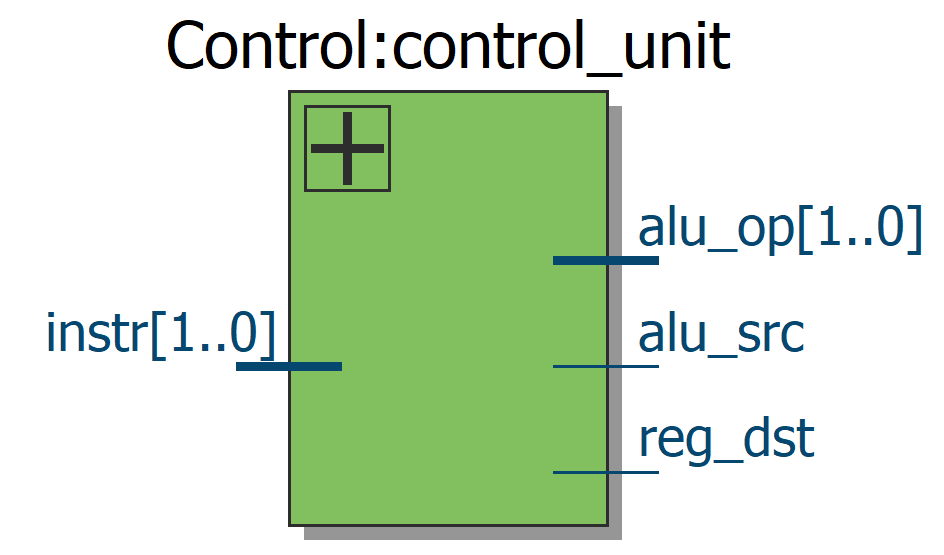
\includegraphics[width=2in]{control_unit.png}
	\caption{Control Unit.}
	\label{fig:cu} 
	\end{center}
\end{figure}

\subsubsection{Mux0}
Mux0 will decide whether the \mintinline{vhdl}{rd_addr} input to the Register 
File will come from the \mintinline{vhdl}{rt_addr} output or 
\mintinline{vhdl}{rd_addr} output of the Instruction Memory. If the 
instruction is \mintinline{vhdl}{addi}, then the Register File 
\mintinline{vhdl}{rd_addr} input will come from the \mintinline{vhdl}{rt_addr} 
output of the Instruction Memory (See Figure \ref{fig:redhorse500}).

\begin{listing}[H]
\caption{Interface to Mux0.}
\label{code:mux0}
\begin{minted}[frame=single,framesep=10pt]{vhdl}
entity mux0 is
  port(
    sel : in std_logic;                      -- select destination address
    a   : in std_logic_vector(1 downto 0);   -- source register address
    b   : in std_logic_vector(1 downto 0);   -- default destination address
    y   : out std_logic_vector(1 downto 0)   -- destination address
  );
end mux0;
\end{minted}
\end{listing}

\subsubsection{Mux1}
Mux1 will decide whether the \mintinline{vhdl}{rt} input to the ALU will come 
from register \mintinline{vhdl}{rt_addr} or from the sign-extended immediate 
value if the instruction is \mintinline{vhdl}{addi}(See Figure 
\ref{fig:redhorse500}).

\begin{listing}[H]
\caption{Interface to Mux1.}
\label{code:mux1}
\begin{minted}[frame=single,framesep=10pt]{vhdl}
entity mux1 is
  port(
    sel : in std_logic;                      -- select data
    a   : in std_logic_vector(7 downto 0);   -- default data
    b   : in std_logic_vector(7 downto 0);   -- data from instruction
    y   : out std_logic_vector(7 downto 0)   -- data out
  );
end mux1;
\end{minted}
\end{listing}


\subsubsection{Sign Extend}
If the instruction is \mintinline{vhdl}{addi}, then the 2-bit immediate value 
which is from the 
\mintinline{vhdl}{rd_addr} output of the Instruction Memory will be converted 
to 8 bits before being passed to the ALU which perform operations on 8-bit 
values.
\begin{listing}[H]
\caption{Interface to Sign Extend.}
\label{code:sign_extend}
\begin{minted}[frame=single,framesep=10pt]{vhdl}
entity sign_extend is
  port(
    data_in  : in std_logic_vector(1 downto 0);
    data_out : out std_logic_vector(7 downto 0)
  );
end sign_extend;
\end{minted}
\end{listing}

\subsubsection{Simulation}
Figure \ref{fig:sim} shows the simulation with the red vertical bar marking the 
execution of the instruction in line 4 of Listing \ref{code:im_code}.

\begin{figure}[H]
	\begin{center}
	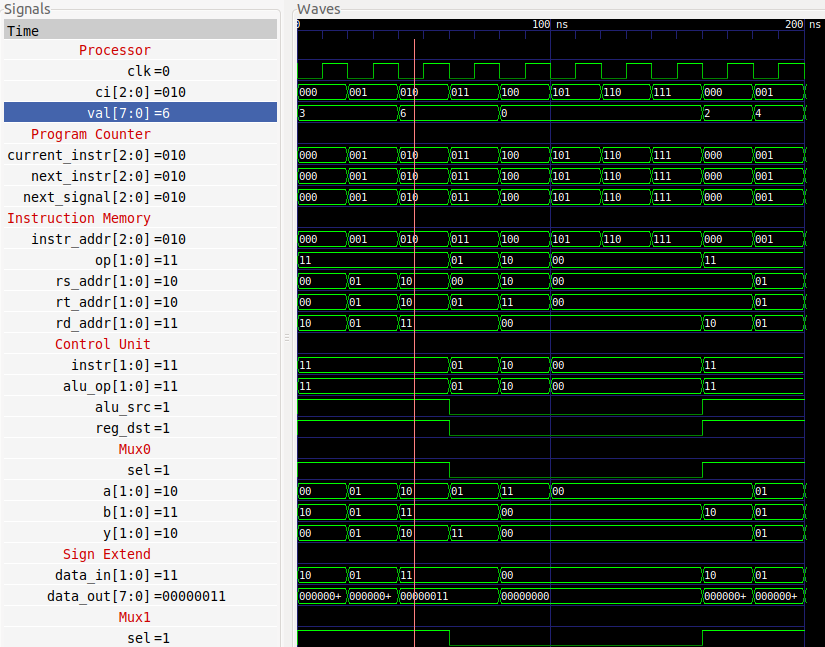
\includegraphics[width=6in]{sim.png}
	\caption{Simulation run of REDHORSE 500.}
	\label{fig:sim} 
	\end{center}
\end{figure}


\section{Summary}
In this lab, you learned that ISAs enable programmers to program the processor 
without knowing the low-level hardware implementation details. It also allows 
multiple vendors to develop different implementations with provide varying  
performance characteristics and cost. You also learned that an ISA when 
combined with operating system services provides an ABI that allow application 
programmers to write programs that will run for a given operating system 
supporting a specific processor.

You were also introduced to the simple TOMA ISA and its implementation, 
REDHORSE 500.

\section{Learning Activities}
Download the source codes for this lab then try experimenting by adding more 
test cases in the testbenches. Submit a PDF document that shows screenshots of 
your modifications and runs. 

\section{Self-Assessment Questions}
\begin{enumerate}
\item What is the main purpose of clocks in sequential circuits?
\item What is the difference between a clocked latch and a flip-flop?
\item Why can't a multiplexer be used in RAM?
\item Why is SRAM more expensive than DRAM?
\item If my CPU is clocked at 800 MHz, what is the period?
\end{enumerate}


\section{Deliverable}
Your final deliverable for this lab is implement the RAM in Figure 
 \ref{fig:sram3}. Submit the VHDL code including a testbench as well as images 
of the waveforms. NOTE: Enable lines should be connected to the output of the 
decoder and the rightmost Din in the figure should be Din[0].


%\begin{thebibliography}{9}
%\end{thebibliography}

\bibliographystyle{unsrt}
\bibliography{toma}
\nocite{*}

\end{document}